\documentclass[a4paper,11pt]{article}

\usepackage[utf8]{inputenc}
\usepackage[sc]{mathpazo}

\usepackage{array}
\usepackage{amsmath}
\usepackage{mathtools}
\usepackage{graphicx}
\usepackage{float}
\usepackage{makeidx}

\graphicspath{./figures}

\title{02286 Logic in Computer Science, Artificial Intelligence and Multi-agent Systems }
\author{
Christian Gram Kalhauge s093273 \\
Andreas Frøsig s093264 \\
Kenneth Balsiger Andersen s093252
}

\makeindex

\begin{document}


\maketitle

\part{Important Notation}

\paragraph{Notation}

\part{Classical Logic (45\%)}

\section{Propositional  Logic}

\subsection{Definition}

\begin{equation}
  \label{eq:1}
  \phi := p \vert \lnot \phi \vert \phi \lor \phi
\end{equation}

Where $p$ is a proposition \index{proposition}. A proposition is logical variable that can hold the values $\top$ or $\bot$.

\subparagraph{Examples on propositions}

\begin{itemize}
\item Your mom is fat!
\item The Moon is made of cheese!
\end{itemize}

\paragraph{Rules}

Where $p$ is a proposition.

\begin{equation}
  \begin{matrix}
    \lnot \lnot p & \mathbf{iff} &p \\
  \end{matrix}
\end{equation}

\paragraph{Derived Notation}

\begin{equation}
  \label{equ:notation-prop}
  \begin{matrix}
   \phi \land \phi & \mathbf{iff} & \lnot ( \lnot \phi \lor \lnot \phi ) \\
   \phi \to \phi & \mathbf{iff} & \lnot \phi \lor \phi \\ 
   \phi  \leftrightarrow \phi & \mathbf{iff}& \phi \lor \phi \\ 
  \end{matrix}
\end{equation}


\paragraph{Recap}

\begin{figure}[H]
  \centering
  \begin{tabular}{lcc}
    \textsc{name} & \textsc{in language} & \textsc{notation} \\\hline
    negation & not A & $\lnot A$ \\ \hline
    conjunction & A and B & $A \land B$ \\ \hline
    disjunction & A or B & $A \lor B$ \\ \hline
    implication & if A then B & $A \to B$ \\ \hline
    biconditional & B if and only if A & $A \leftrightarrow B$ \\ \hline

  \end{tabular}
  \caption{Description of notation}
  \label{fig:propositional}
\end{figure}


\subsection{Derived Definitions}

\paragraph{Literal}
A literal is a propositional constant or variable or its negation. 


\paragraph{Elementary disjunction or conjunction}
Is a disjunction or conjunction of one or more literals.

\subsection{Forms}

Every propositional formula is equivalent to a disjunctive normal form and to a conjunctive normal form

\paragraph{Conjunctive normal form (CNF)}

Is a logical propsitional formula where we conjunct one or more elementary disjunctions. And's outside and Or's inside.

\subparagraph{Examples}

\begin{itemize}
\item $(p \lor q) \land (\neg p \lor q)$
\end{itemize}

\paragraph{Disjunctive normal form (DNF)}

Same as CNF but have Or's outside and And's inside.

\subparagraph{Examples}

\begin{itemize}
\item $(p \land q) \lor (\neg p \land q)$
\end{itemize}

\paragraph{Algorithm to transform into CNF /DNF}

\begin{itemize}
\item Eliminate all occurrences of $\leftrightarrow$ and $\to$ using the equivalence  from \ref{equ:notation-prop}.
\item Transform to negation normal form by using the relevant equivalences. 
\end{itemize}

%%% Local Variables: 
%%% mode: latex
%%% TeX-master: "../../Notes"
%%% End: 

\documentclass[10pt,a4paper]{article}
\usepackage[utf8]{inputenc}
\usepackage{amsmath}
\usepackage{amsfonts}
\usepackage{amssymb}
\usepackage{fullpage}
\usepackage{array}
\begin{document}
	\subsection{Natural Deduction}
	\subsubsection{Rules}
	{
	\begin{tabular}{m{3cm} p{4cm} m{3cm} p{4cm}}
		
		Introduction rules: & meaning	& Elimination rules & meaning\\ 
		$ \left( \land I\right) \frac{A,B}{A\land B} $ & \normalsize if we have concluded A and B separately vi can conclude A and B	& $\left( \land E\right) \frac{A \land B}{A}, \frac{A \land B}{B} $ & \normalsize if we have B and A we know A must be true  \\[1cm]  
		\hline
		$ \left( \lor I\right) \frac{A}{A\lor B} , \frac{B}{A\lor B} $ & \normalsize if we have A we can introduce B & $(\lor E) \frac{A \lor B \begin{matrix}
			[A] & [B]  \\
			\vdots & \vdots  \\
			C & C
			\end{matrix}}{C} $ & \normalsize If by assuming A and B both can derive C and we know that A or B is true we can conclude C
		
		\\[1cm]
		\hline
		$(\to I) \frac{\begin{matrix}
			[A]  \\
			\vdots   \\
			B 
			\end{matrix}}{A\to B} $ & \normalsize if we by assuming A gets a B we can conclude that A implies B & $ (\to E) \frac{A,A\to B}{B} $ & if we know A an that A implies B we can conclude B \\[1cm] 
		\hline
		$ (\neg I) \frac{\begin{matrix}
			[\neg A]  \\
			\vdots   \\
			\bot 
			\end{matrix}}{\neg A} $ & \normalsize if we assume A and reaches a falsum we can conclude that A is not the case & $ (\neg E) \frac{A,\neg A}{\bot} $ & if we reach a A and $ \neg $A we can conclude a falsum\\[1cm]
		\hline
		Ex falsum quodlibet & & Reductio ad absurdum:\\ 
		$ (\bot ) \frac{\bot}{A} $ & from a falsum anything can be derived & $ (RA) \frac{\begin{matrix}
			[\neg A]  \\
			\vdots   \\
			\bot 
			\end{matrix}}{A} $ & direct opposed of $ \neg I $
	
	\end{tabular}
	\subsubsection{Syntax}
	important notes for syntax:
	\begin{itemize}
		\item $ []^x $ around assumptions where x is the number of the assumption
		\item name of the rule used at the left og the fraction line; $$ \left( \lor I\right) \frac{A}{A\lor B} $$
		\item name the number of the assumption you neutralize at the right of the fraction line:$$\frac{A}{A\lor B}x $$
		\item assumptions can be introduced when ever you want, but only removed is a rule allow it ( $ \neg I $ ) and all assumptions must be used in the end($ \to I $)
	\end{itemize}
 	
	 
\end{document}




%%% Local Variables: 
%%% mode: latex
%%% TeX-master: "../../Notes"
%%% End: 

\section{First-order  Logic}

\documentclass[10pt,a4paper]{article}
\usepackage[latin1]{inputenc}
\usepackage{amsmath}
\usepackage{amsfonts}
\usepackage{amssymb}
\usepackage{graphicx}
\usepackage{float}
\begin{document}
\section{Semantic Tableaux for first-order logic}

\begin{center}
\textbf{Quantifier rules for Semantic Tableaux}
\end{center}
\begin{tabular}{l c l c}
($ \forall $ T) &  \parbox{5cm}{\centering$ \forall x A(x) : $ T
\newline
$ \downarrow $
\newline
$ A(t/x) : $ T
\newline
for any term \textit{t} occurring on this branch and free for \textit{x} in \textit{A}} & ($ \exists $ T)* & \parbox{5cm}{\centering$ \exists x A(x) : $ T
\newline
$ \downarrow $
\newline
$ A(c/x) : $ T
\newline
for a \textit{new} constant symbol \textit{c} not yet occurring on this branch}  \\[1.5cm]

($ \exists $ F) & \parbox{5cm}{\centering$ \exists x A(x) : $ F
\newline
$ \downarrow $
\newline
$ A(t/x) : $ F
\newline
for any term \textit{t} occurring on this branch and free for \textit{x} in \textit{A}} & ($ \forall $ F)*  & \parbox{5cm}{\centering$ \forall x A(x) : $ F
\newline
$ \downarrow $
\newline
$ A(c/x) : $ F
\newline
for a \textit{new} constant symbol \textit{c} not yet occurring on this branch}  \\
\end{tabular}

(*) \textit{This rule may only be applied once for the given formula on each branch}

Here are some examples of a semantic tableaux with first-order logic \cite[p. 46]{LecPartII}.

\begin{figure}[H]
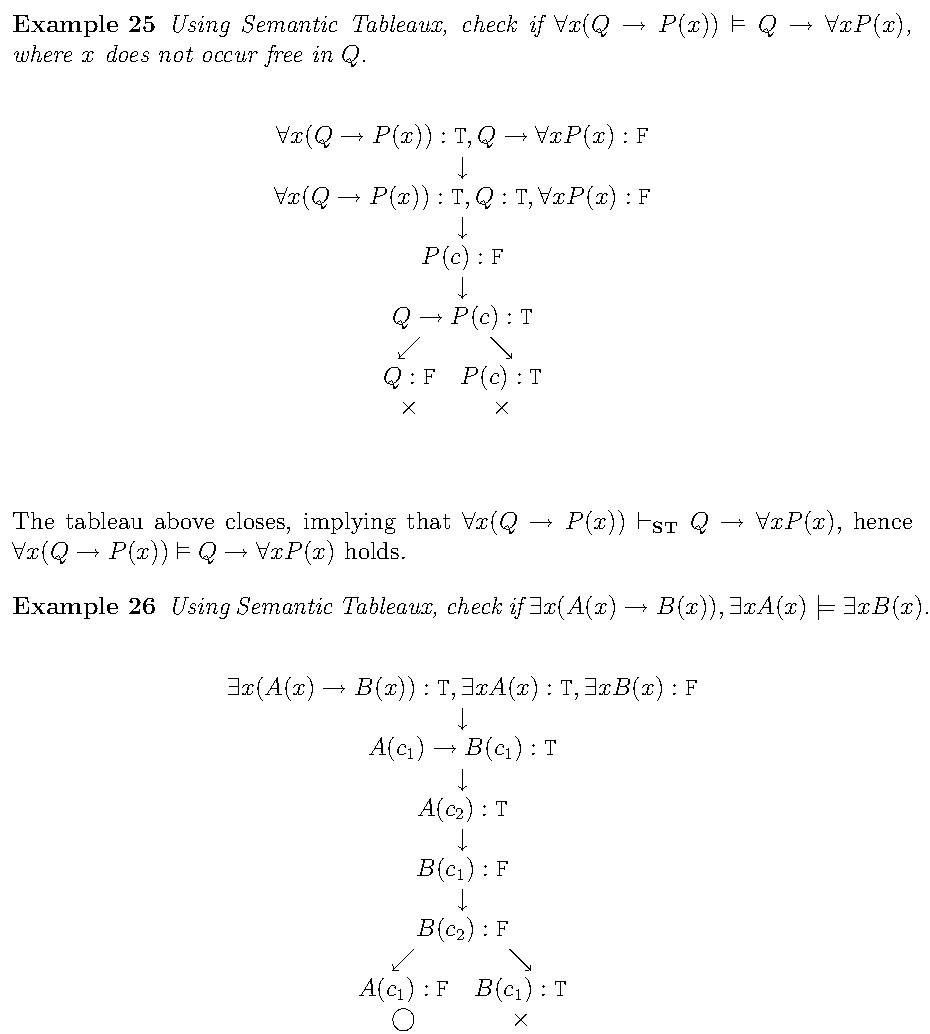
\includegraphics[scale=0.6]{./figures/tableaux.pdf}
\end{figure}

\section{Prenex and clausal normal forms}
\subsection{Negating first-order formulae. Negation normal form}

\textit{Negation normal form}\cite[p.58]{LecPartII} means that negations only occurs in front of atomic formulae. eg:

\begin{figure}[H]
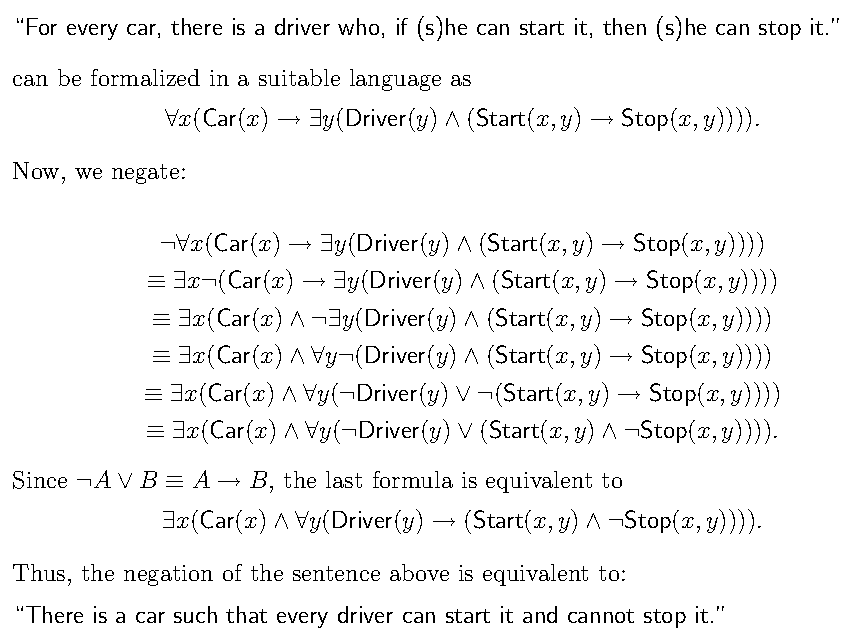
\includegraphics[scale=0.6]{./figures/negnormform.pdf}
\end{figure}

\subsection{Prenex normal forms}

\textit{Prenex normal forms} \cite[p. 59]{LecPartII} refer to a form of the formula where all the quantifications have been moved to the outermost scope like:
$$ Q_1 x_1 .. Q_n x_n A $$

where $ Q_n $ is all the quantifiers called the \textbf{prefix} and $ A $ is the formula called the \textbf{matrix}

If the formula itself is in either CNF or DNF then we refer to the formula as a \textit{prenex CNF / PCNF} or \textit{prenex DNF / PDNF}

\textbf{Algorithm for construction these normal forms:}

\begin{enumerate}
\item Eliminate all occurences of $ \to $ and $ \leftrightarrow $ as in the propositional case.
\item Import all negations inside all other logical connectives and transform the formula to negation normal form.
\item Pull all quantifiers in front and thus transform the formula into a prenex form.

For that use the equivalences:
      \begin{enumerate}
\item $ \forall x P \land \forall x Q \equiv \forall x(P \land Q) $
\item $ \exists x P \lor \exists x Q \equiv \exists(P \lor Q) $

to pull some quantifiers outwards and, after renaming the formula \textit{wherever necessary}.

Then, use also the following equivalences, where \textit{x} does not occur free in \textit{Q}, until the formula is transformed to a prenex form:

\item $ \forall x P \land Q \equiv Q \land \forall x P \equiv \forall x(P\land Q) $
\item $ \forall x P \lor Q \equiv Q \lor \forall x P \equiv \forall x(P \lor Q) $
\item $ \exists x P \lor Q \equiv Q \lor \exists x P \equiv \exists x (P \lor Q) $
\item $ \exists x P \land Q \equiv Q \land \exists x P \equiv \exists x(P\land Q) $
\end{enumerate}
\item Finally, transform the matrix in a DNF or CNF, just like a propositional formula.
\end{enumerate}

Here are some examples:
\begin{figure}[H]
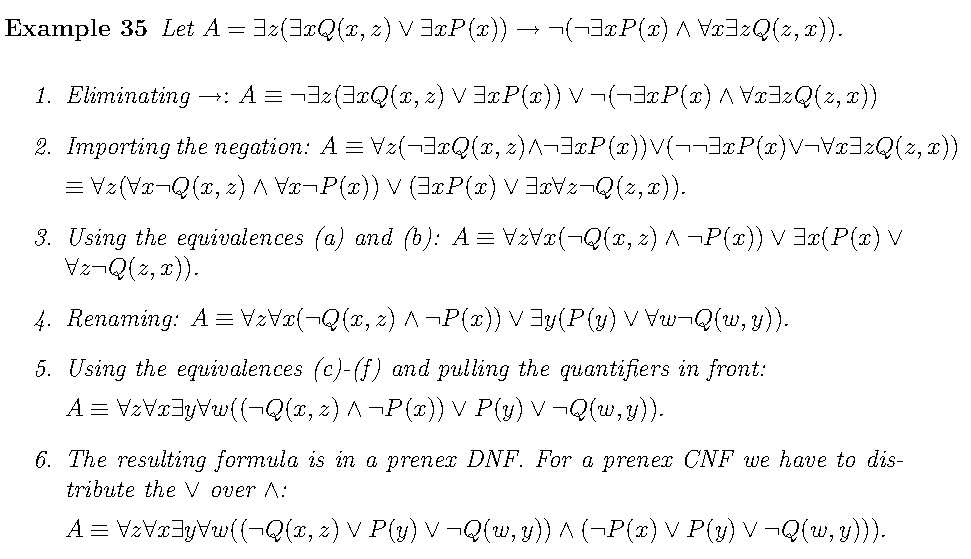
\includegraphics[scale=0.6]{./figures/prenexex.pdf}
\end{figure}

\subsection{Skolemization}

Skolemization\cite[p. 60]{LecPartII} is a procedure used to eliminate the existential quantifiers in a first-order formula in a prenex form by a uniform replacement of all occurrences of existentially
quantified individual variables with terms headed by new functional symbols, called
\textit{Skolem functions}.\\

\textit{Skolem functions} take as arguments all variables (if any) which are bound by universal quantifiers in the scope of which the given existential quantifier sits. In particular, existentially quan-
tified variables not in the scope of any universal quantifiers are replaced by constant symbols, called \textit{Skolem constants}.

\textbf{Examples of skolemization}
\begin{figure}[H]
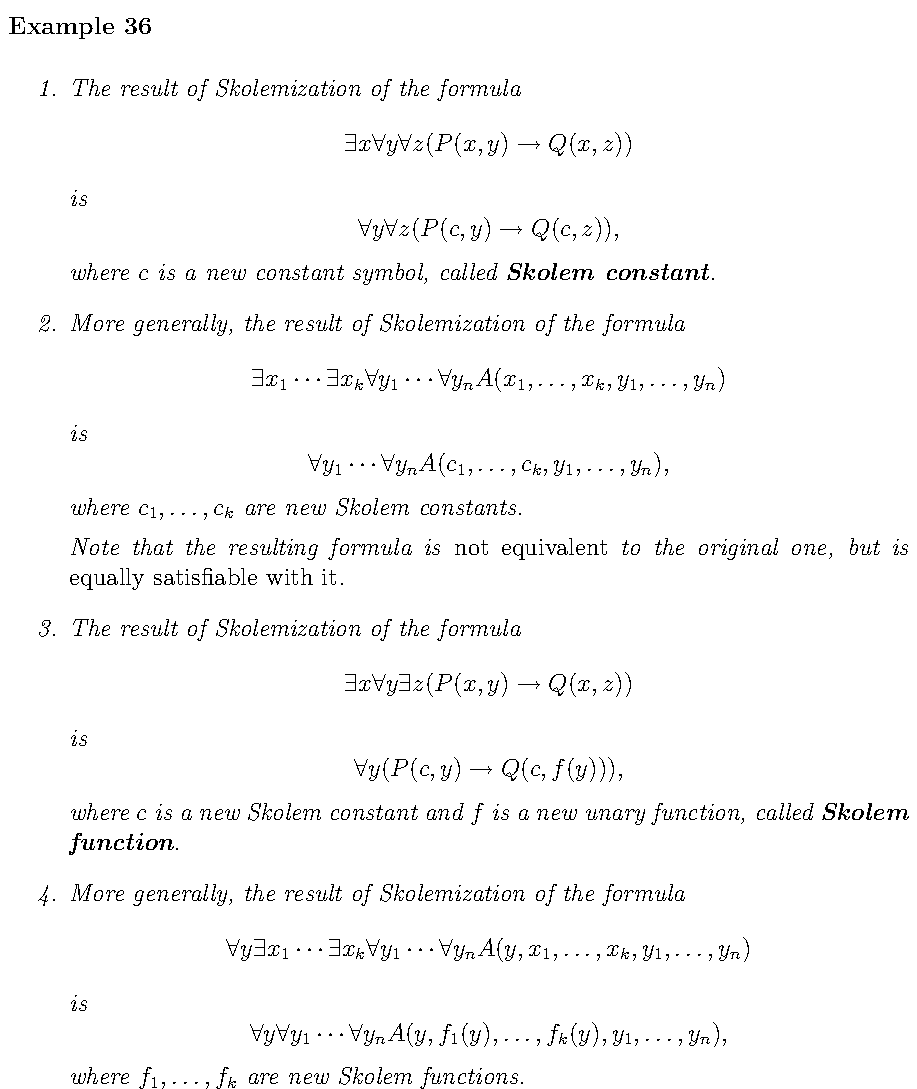
\includegraphics[scale=0.6]{./figures/skolemex1.pdf}
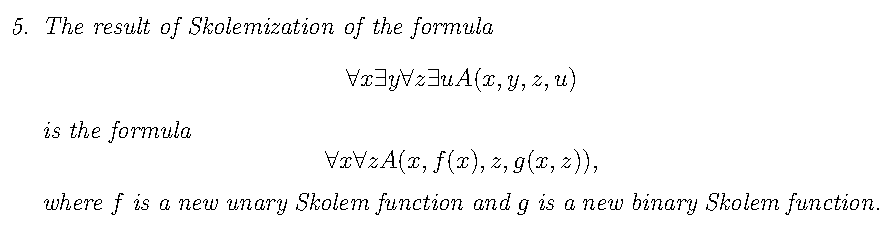
\includegraphics[scale=0.6]{./figures/skolemex2.pdf}
\end{figure}


\subsection{Clausal form}

\textit{Clausal forms} \cite[p. 62]{LecPartII} is a set of \textit{literals} (representing their disjunction).

All clauses are implicitly assumed to be universally quantified.

\textbf{The algorithm for transforming any formula into clausal form}

\begin{itemize}
\item Transform \textit{A} into prenex CNF
\item Skolemize all existential quantifiers.
\item Remove all universalt quantifiers.
\item Wrute the \textit{matrix} (which is in CNF) as a set of clauses.
\end{itemize}

\begin{figure}[H]
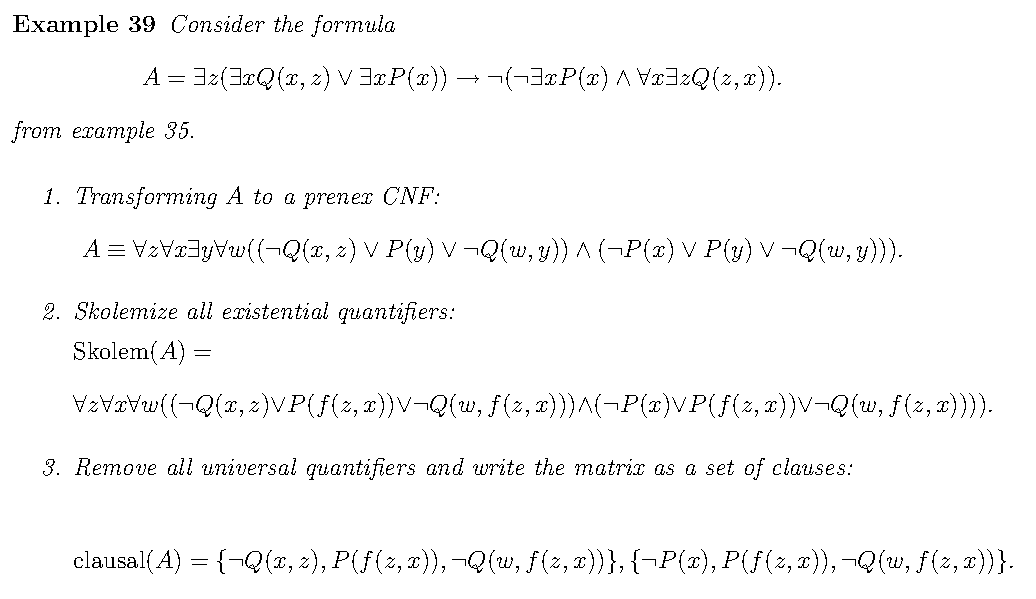
\includegraphics[scale=0.6]{./figures/clausalex.pdf}
\end{figure}

\end{document} 

\part{Non-Classical Logic (55\%)}


\part{Extra}

\printindex


\nocite{*}

\bibliography{logic}
\bibliographystyle{amsalpha}


\end{document}


%%% Local Variables: 
%%% mode: latex
%%% TeX-master: t
%%% End: 
